
% =========================================================================
% CHAPTER THREE: TOOLS AND EQUIPMENT USED
% =========================================================================
\section{Introduction}
This chapter describes and presents a comprehensive overview of the tools, the hardware components, measurement instruments, and software tools ``platforms'' that were used and utilized to design, build, test, and operate the solar-powered electric vehicle (EV) charging station. The equipment is categorized according to its functional role within the overall system architecture.

In this chapter, we present the key tools, equipment, and instruments utilized in the process of hardware development, prototyping, testing, and validation of our solar-powered electric vehicle (EV) charging station project. The effective implementation of this project depended not just on correct circuit design and simulation but also on the judicious selection and application of laboratory instruments and measurement systems that guaranteed reliability, repeatability, and safety.

The equipment outlined in this chapter were of paramount importance during several stages of the project, including PCB soldering, component mounting, waveform measurement, and power testing. Each piece of equipment was selected based on its specifications, its suitability to work with power electronics systems, and its ability to enable a smooth workflow throughout the process of assembling and verifying circuits. This chapter describes the technical role played by each device, identifies the reason for inclusion, and defines its particular contribution to the success of the practical implementation of Solar Photovoltaic (PV) Panels, DC-DC converters, and Battery Energy Storage Systems that form the fundamental building blocks of solar-powered electric vehicle (EV) charging station system.

% =========================================================================
% SECTION 3.2: POWER SUPPLY & DISTRIBUTION DEVICES
% =========================================================================
\section{Power Supply \& Distribution Devices}

\subsection{Programmable DC Power Supply (TDK-Lambda GEN 300-11)}

\subsubsection{Tool Overview}
The TDK-Lambda GEN 300-11 is a programmable DC power supply from the GENESYS\texttrademark\ series, known for its high performance, reliability, and precision in laboratory and industrial environments. This specific model provides an output range of 0--300 V DC and up to 11 A of output current, making it suitable for medium to high-power applications in power electronics testing. The unit supports both manual control via its front panel and remote control through analog or digital interfaces such as RS-232, GPIB, or LAN. Its front panel allows precise voltage and current adjustment using rotary encoders, as well as monitoring via digital display.

\begin{figure}[H]
    \centering
    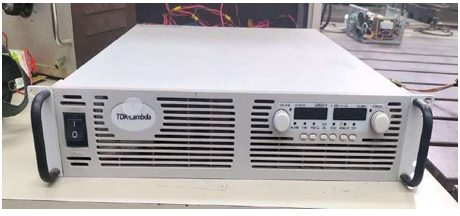
\includegraphics[width=0.75\textwidth]{Figures/Figure 3.1.png}
    \caption{TDK-Lambda GEN 300-11 Programmable DC Power Supply.}
    \label{fig:tdk_lambda}
\end{figure}

\subsubsection{Key Specifications}
\renewcommand{\arraystretch}{1.3}
\rowcolors{2}{white}{gray!8}
\begin{tabularx}{\textwidth}{>{\bfseries}X l}
    \toprule
    Parameter & Specification \\
    \midrule
    Model & TDK-Lambda GEN 300-11 \\
    O/P Voltage Range & 0--300 V DC \\
    O/P Current Range & 0--11 A \\
    Power Output & Up to 3.3 kW \\
    Interface & Local + Remote (RS-232, GPIB, LAN) \\
    Protection Features & Overvoltage, Overcurrent, Foldback, Overtemperature \\
    \bottomrule
\end{tabularx}

\subsubsection{Role in the Graduation Project}
This programmable DC power supply was a critical component in the hardware validation of the solar-powered electric vehicle (EV) charging station circuits. Its ability to provide a precisely regulated and adjustable DC voltage allowed for the safe and repeatable powering of various converter topologies implemented during the project.

Specifically, it was used to:
\begin{itemize}
    \item Power the DC-DC converter circuits (Buck, Boost, Buck-Boost) under controlled conditions.
    \item Test different duty cycles and load conditions by adjusting input voltage dynamically.
    \item Ensure stable and isolated DC input, mimicking real-world conditions without the hazards of using high-voltage batteries during early testing phases.
\end{itemize}

% =========================================================================
% SECTION 3.3: MEASUREMENT & MONITORING INSTRUMENTS
% =========================================================================
\section{Measurement \& Monitoring Instruments}

\subsection{Digital Storage Oscilloscope - Hantek DSO4254B}

\subsubsection{Tool Overview}
The Hantek DSO4254B is a 4-channel Digital Storage Oscilloscope (DSO) widely used in electrical engineering laboratories for capturing, visualizing, and analyzing electrical waveforms. With a bandwidth of 250 MHz and a real-time sampling rate of up to 1 GSa/s, it is suitable for diagnosing both low- and high-frequency signals in power electronics applications. This oscilloscope offers precise control over vertical and horizontal axes, trigger settings, and math operations, making it highly adaptable for testing converters, inverters, and complex switching circuits like those found in solar-powered electric vehicle (EV) charging stations.

\begin{figure}[H]
    \centering
    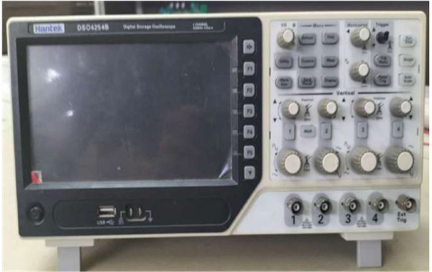
\includegraphics[width=0.7\textwidth]{Figures/Figure 3.2.png}
    \caption{Hantek DSO4254B Digital Storage Oscilloscope.}
    \label{fig:hantek_oscilloscope}
\end{figure}

\subsubsection{Key Specifications}
\renewcommand{\arraystretch}{1.4} % Slightly more breathing room
\rowcolors{2}{white}{gray!8} 

\begin{tabularx}{\textwidth}{>{\bfseries}l X} % <-- Changed first to 'l' and second to 'X'
    \toprule
    Parameter & Specification \\
    \midrule
    Model & Hantek DSO4254B \\
    Channels & 4 (CH1--CH4) + External Trigger (Ext Trig) \\
    Bandwidth & 250 MHz \\
    Real-time Sampling Rate & 1 GSa/s \\
    Display & Large color LCD screen \\
    Ports & USB Host, USB Device, LAN \\
    Functions & Waveform generator, cursor measurements, auto-set, FFT analysis, save/recall \\
    \bottomrule
\end{tabularx}

\subsubsection{Role in the Graduation Project}
This oscilloscope was indispensable in verifying the performance and stability of the entire power conversion system used in the solar-powered electric vehicle (EV) charging station. It provided real-time, high-resolution visibility into the behavior of voltage and current waveforms across different stages of the circuit, including:
\begin{itemize}
    \item DC-DC converter output ripple measurements and transient response.
    \item Switching behavior analysis for MOSFETs and IGBTs in the Buck, Boost, and Buck-Boost circuits.
    \item Gate signal validation from the control circuit and drivers.
    \item Startup and shutdown transients during power sequencing tests.
\end{itemize}
The ability to visualize waveform distortion, harmonics, and frequency behavior was essential for matching simulation results from MATLAB/Simulink with physical circuit behavior, ensuring accurate hardware validation.

\subsubsection{Importance in Achieving Project Goals}
Without this oscilloscope, it would not have been possible to:
\begin{itemize}
    \item Confirm switching frequency adherence and waveform shape.
    \item Validate converter efficiency by analyzing voltage/current overlap.
    \item Identify noise or instability issues in real time.
    \item Troubleshoot signal integrity during integration between stages.
\end{itemize}

\subsection{Oscilloscope - DSO 138}
\subsubsection{Tool Overview}
It was very practical for home testing when the laboratory was not reachable.
\begin{figure}[H]
    \centering
    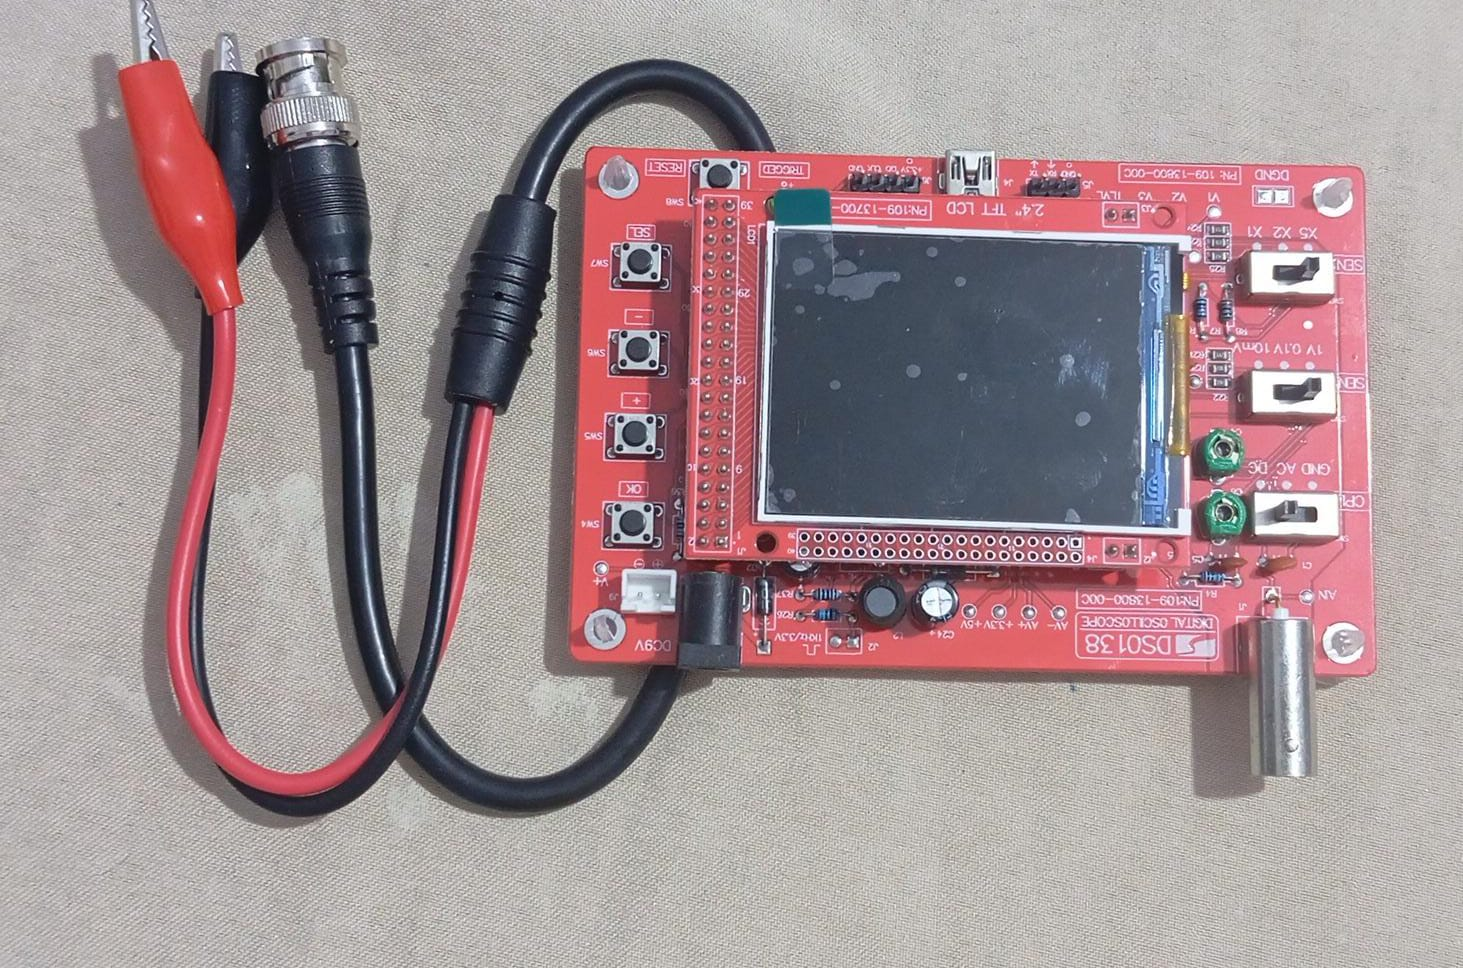
\includegraphics[width=0.7\textwidth]{Figures/Figure 3.3.jpeg}
    \caption{DSO 138 Oscilliscope}
    \label{fig:multimeter}
\end{figure}


% -------------------------------------------------------------------------
\subsection{Digital Multimeter - UNI-T UT33D+}

\subsubsection{Description}
The UNI-T UT33D+ is a handheld digital multimeter used for measuring a variety of electrical parameters. It is part of the UT33+ series, known for affordability and reliability in lab and educational settings. This particular model supports both AC and DC voltage, current, resistance, diode testing, and continuity checking, and includes a non-contact voltage (NCV) detection function for live wire sensing.

\begin{figure}[H]
    \centering
    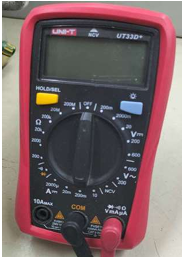
\includegraphics[width=0.35\textwidth]{Figures/Figure 3.4.png}
    \caption{UNI-T UT33D+ Digital Multimeter.}
    \label{fig:multimeteer}
\end{figure}

\subsubsection{Key Features}
\renewcommand{\arraystretch}{1.4} % Nice breathing room between rows
\rowcolors{2}{white}{gray!8} % Alternating soft gray zebra stripes

\begin{tabularx}{\textwidth}{>{\bfseries}l X}
    \toprule
    Feature Category & Technical Specification \\
    \midrule
    Voltage Measurement & AC/DC Voltage up to 600 V \\
    Current Measurement & DC Current up to 10 A (utilizing the dedicated 10A MAX port) \\
    Resistance Measurement & Resistance range up to 20 M$\Omega$ \\
    Testing Functions & Integrated diode testing and circuit continuity checking \\
    Safety \& Convenience & Non-Contact Voltage (NCV) detection, manual range selection, display hold function, backlit display, and fused inputs (250V/200mA and 250V/10A) \\
    \bottomrule
\end{tabularx}

\newpage

% -------------------------------------------------------------------------
\subsection{Voltage Sensor Module – DC 0-25V}

\subsubsection{Description}
The voltage sensor module is a compact board based on a resistive voltage divider, used to scale down DC voltages so they can be safely read by a microcontroller's analog input. Since the Arduino's analog pins can only accept up to 5V, this module allows voltages as high as 25V to be measured indirectly by reducing the input by a fixed factor before it reaches the analog pin.

\begin{figure}[H]
    \centering
    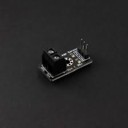
\includegraphics[width=0.45\textwidth]{Figures/Figure 3.5.jpg}
    \caption{DC 0--25V Voltage Sensor Module.}
    \label{fig:voltage_sensor}
\end{figure}

\subsubsection{Key Specifications}
\renewcommand{\arraystretch}{1.4} % Nice breathing room between rows
\rowcolors{2}{white}{gray!8} % Alternating soft gray zebra stripes

\begin{tabularx}{\textwidth}{>{\bfseries}l X}
    \toprule
    Parameter & Specification \\
    \midrule
    Type & Resistive Voltage Divider Sensor Module \\
    Voltage Input Range & DC 0--25 V \\
    Divider Ratio & 5:1 \\
    Divider Resistors & 30 k$\Omega$ and 7.5 k$\Omega$, 1\% tolerance \\
    Voltage Detection Resolution & 0.00489 V \\
    Key Function & Scales down higher DC voltages to a safe 0--5V range for analog measurement by a microcontroller \\
    \bottomrule
\end{tabularx}

\newpage

\subsubsection{Application in the Project}
In this project, the voltage sensor module is used to measure DC voltage at key points in the circuit, such as the PV array output and battery terminal voltage, by scaling the measured voltage down by a factor of 5 before feeding it into the Arduino Uno's analog input. This scaled voltage reading allows the Arduino to reconstruct the actual voltage value in software and use it, alongside the ACS712 current sensor reading, for the MPPT algorithm's power calculation and duty-cycle adjustment, as well as for monitoring battery voltage during charge/discharge control.

% -------------------------------------------------------------------------
\subsection{Current Sensor – ACS712 (5A)}

\subsubsection{Description}
The ACS712 is a fully integrated, Hall-effect-based linear current sensor IC that measures both AC and DC current and converts it into a proportional analog voltage output. Since it senses current through a magnetic field rather than a direct electrical connection, it provides galvanic isolation between the high-current path being measured and the low-voltage signal/control circuitry, making it safe to interface directly with a microcontroller's analog input.

\begin{figure}[H]
    \centering
    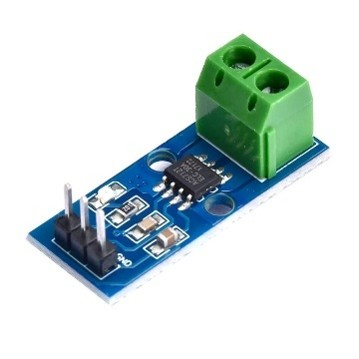
\includegraphics[width=0.45\textwidth]{Figures/Figure 3.6.jpg}
    \caption{ACS712 5A Current Sensor Module.}
    \label{fig:current_sensor}
\end{figure}

\subsubsection{Key Specifications}
\renewcommand{\arraystretch}{1.4} % Nice breathing room between rows
\rowcolors{2}{white}{gray!8} % Alternating soft gray zebra stripes

\begin{tabularx}{\textwidth}{>{\bfseries}l X}
    \toprule
    Parameter & Specification \\
    \midrule
    Manufacturer & Allegro MicroSystems \\
    Type & Hall-Effect Linear Current Sensor IC (module/breakout board) \\
    Model & ACS712ELC-05A (5A variant) \\
    Measurement Range & $-5$ A to $+5$ A (bidirectional) \\
    Sensitivity & 180--190 mV/A, typically 185 mV/A \\
    Supply Voltage & 4.5 V to 5.5 V DC \\
    Zero-Current Output Voltage & $V_{CC}/2$ (2.5 V at 5V supply) \\
    Isolation & 2.4 kV$_{RMS}$ isolation \\
    Key Function & Converts measured DC/AC current into a proportional analog voltage signal for monitoring or feedback control \\
    \bottomrule
\end{tabularx}

\subsubsection{Application in the Project}
In this project, the ACS712 5A current sensor measures current at key points—such as PV array output and battery charge/discharge current—and feeds the corresponding analog voltage signal to the Arduino's analog input. This current feedback is essential to the MPPT algorithm, which uses it alongside voltage readings to calculate PV power and adjust the duty cycle accordingly, and also supports safe charge/discharge current regulation for the battery.

% =========================================================================
% SECTION 3.4: LOAD SIMULATION DEVICES (BATTERIES)
% =========================================================================
\section{Load Simulation Devices (Batteries)}

\subsection{EV Battery Simulator (IMR14500 Lithium-Ion Pack)}

\subsubsection{Description}
The battery used to simulate the electric vehicle in this project consists of two IMR14500 lithium-ion cells, each rated 3.7V 800mAh, connected in series to form a 7.4V nominal pack. The IMR14500 is a rechargeable lithium-manganese cell in the AA-size (14500) format, designed for stable power delivery, fast charging, and long cycle life, making it suitable as a compact, scaled-down stand-in for an EV battery in laboratory testing.

\begin{figure}[H]
    \centering
    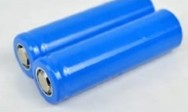
\includegraphics[width=0.6\textwidth]{Figures/Figure 3.7.jpg}
    \caption{Lithium-Ion Battery Pack (IMR14500 Cells in 2S Configuration).}
    \label{fig:ev_battery_pack}
\end{figure}

\subsubsection{Key Specifications}
\renewcommand{\arraystretch}{1.4} % Provides clean vertical padding
\rowcolors{2}{white}{gray!8} % Alternating soft gray zebra stripes

\begin{tabularx}{\textwidth}{>{\bfseries}l X}
    \toprule
    Parameter & Specification \\
    \midrule
    Cell Type & IMR14500 Lithium-Ion (Lithium-Manganese chemistry) \\
    Cell Size & 14500 (AA-size format) \\
    Nominal Voltage per Cell & 3.7 V \\
    Capacity per Cell & 800 mAh (actual capacity) \\
    Configuration & 2 cells in series (2S) \\
    Nominal Pack Voltage & 7.4 V \\
    Pack Capacity & 800 mAh (capacity unchanged in series connection; only voltage adds) \\
    Charge Cut-off Voltage & Typically 4.2 V per cell (pack total: 8.4 V) \\
    Discharge Cut-off Voltage & Typically 3.0 V per cell (pack total: 6.0 V) \\
    Key Function & Acts as a scaled-down model of an electric vehicle battery for laboratory testing \\
    \bottomrule
\end{tabularx}

\subsubsection{Application in the Project}
In this project, the 2S IMR14500 3.7V 800mAh lithium-ion battery pack is used to simulate an electric vehicle's battery during laboratory testing, representing the load to be charged by the PV-based charging station. This allows the charging behavior of the system—including the converter stages and control algorithm—to be validated on a small scale, safely standing in for an actual EV battery pack.

% -------------------------------------------------------------------------
\subsection{Stationary Battery Storage System (ICR18650 Pack with BMS)}

\subsubsection{Description}
The energy storage battery used in this project (for storing PV energy when no EV is connected) consists of two ICR18650 lithium-ion cells connected in series, paired with an HW-391 battery management system (BMS) protection board. The BMS monitors and protects the cell pack during charge and discharge, preventing overcharge, over-discharge, and overcurrent conditions that could otherwise damage the cells or create safety hazards.

\begin{figure}[H]
    \centering
    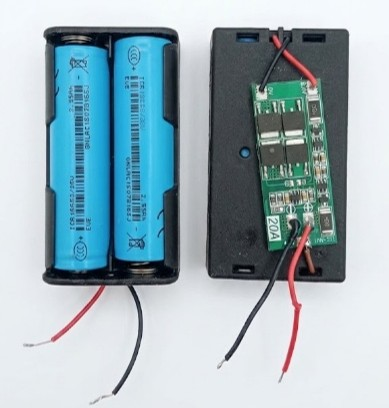
\includegraphics[width=0.35\textwidth]{Figures/Figure 3.8.jpg}
    \caption{ICR18650 Battery Storage Pack with Integrated Protection Board Layout.}
    \label{fig:storage_battery_pack}
\end{figure}

\subsubsection{Key Specifications}
\renewcommand{\arraystretch}{1.3}
\rowcolors{2}{white}{gray!8}
\begin{tabularx}{\textwidth}{X X}
    \toprule
    \textbf{Battery Cells Component} & \textbf{BMS Protection Board (HW-391)} \\
    \midrule
    Manufacturer: EVE Energy & Model: HW-391 \\
    Cell Type: ICR18650 Lithium-Ion (18650 cylindrical format) & Configuration: 2S Li-ion protection board \\
    Nominal Voltage per Cell: 3.7 V & Maximum Discharge Current: 20 A \\
    Capacity per Cell: 2.55 Ah (2550 mAh) & Charge Cut-off Voltage: 8.4 V (4.2 V per cell) \\
    Configuration: 2 cells in series (2S) & Discharge Cut-off Voltage: $\sim$6.0 V (3.0 V per cell) \\
    Nominal Pack Voltage: 7.4 V & Key Function: Overcharge, over-discharge, and \\
    Pack Capacity: 2.55 Ah & overcurrent protection for the 2S battery pack \\
    \bottomrule
\end{tabularx}

\newpage

\subsubsection{Application in the Project}
In this project, this 2S ICR18650 battery pack (with integrated BMS) serves as the system's energy storage element, used when no simulated EV is connected to the charging station. It stores excess energy harvested from the PV array through the MPPT-controlled converter stage, allowing the system to continue supplying power when solar generation is intermittent or unavailable. The HW-391 BMS protects the pack during both charging from the PV side and discharging to the load, ensuring the cells operate within safe voltage and current limits throughout testing.

% =========================================================================
% SECTION 3.5: CONTROL DEVICES
% =========================================================================
\section{Control Devices}

\subsection{Arduino Uno Development Board}

\subsubsection{Description}
\begin{itemize}
    \item \textbf{Manufacturer / Series:} Arduino AG / Arduino LLC (Arduino Uno Rev3).
    \item \textbf{Core Processing Hardware:} ATmega328P micro-controller utilizing an 8-bit AVR RISC architecture operating at a clock speed of 16 MHz.
    \item \textbf{Onboard Features:} 14 digital I/O pins (6 of which provide PWM output), 6 analog input pins, and 1 UART (hardware serial) port.
    \item \textbf{Power Options \& Connectivity:} Supports USB programming/communication (5V interface) or external power via DC jack / $V_{in}$ pin ($7$--$12\text{V}$ recommended), equipped with an onboard voltage regulator, reset button, SPI, and $\text{I}^2\text{C}$ interfaces.
\end{itemize}

\begin{figure}[H]
    \centering
    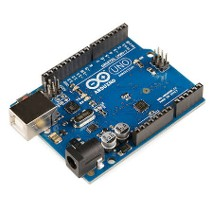
\includegraphics[width=0.5\textwidth]{Figures/Figure 3.9.jpg}
    \caption{Arduino Uno Rev3 Development Board.}
    \label{fig:arduino_uno}
\end{figure}

\subsubsection{Application in the Project}
In this project, the Arduino Uno serves as the central digital controller responsible for generating the switching signals for the power electronic stages in the solar-to-EV-charging system. Since the Uno's PWM outputs are low-power logic-level signals (0--5V), they are not capable of directly driving the power semiconductor switches; therefore, external gate driver ICs are used to amplify and level-shift these signals to the voltage/current levels required to switch the MOSFETs/IGBTs in each converter stage.

\begin{description}
    \item[MPPT Control:] The Arduino reads the PV array's voltage and current through its analog input channels (via voltage/current sensor signals) and runs the Maximum Power Point Tracking algorithm (e.g., Perturb \& Observe or Incremental Conductance) in real time. Based on the computed reference, it generates a PWM duty cycle signal, which is fed through a gate driver IC to drive the MPPT-stage DC-DC converter switch, continuously adjusting the duty cycle to keep the PV array operating at its maximum power point under varying irradiance and temperature.
    \item[Boost Converter Control:] A PWM output channel from the Arduino is passed through a gate driver IC to drive the boost converter switch, regulating the step-up of PV output voltage to the level required by the battery bus or DC link.
    \item[Buck Converter Control:] Another PWM channel, similarly buffered through a gate driver IC, controls the buck converter switching, stepping down the bus voltage to the level required for battery charging or for the EV charging output.
    \item[Two-Quadrant Chopper Control:] The Arduino generates the gating signals for the two-quadrant (bidirectional) chopper; these are routed through dedicated gate driver ICs to drive both switches of the chopper, enabling controlled power flow in both directions—allowing the system to manage battery charging (buck mode) and discharging/power delivery (boost mode) depending on system state.
    \item[Signal Conditioning Interface:] Voltage and current sensor outputs are fed into the Arduino's analog inputs (after appropriate scaling/conditioning circuitry) to enable closed-loop feedback control across all converter stages.
    \item[Gate Driver Interface:] The gate driver ICs serve as the isolation and amplification stage between the Arduino's low-voltage logic outputs and the high-voltage/high-current switching requirements of the power converters, also providing protection against noise and voltage spikes from the power circuit reaching the microcontroller.
\end{description}

% =========================================================================
% SECTION 3.6: BASIC POWER ELECTRONICS COMPONENTS
% =========================================================================
\section{Basic Power Electronics Components}

\subsection{IR2111 – High-Voltage Gate Driver IC}

\subsubsection{Description and Key Specifications}
The IR2111 is a high-voltage, high-speed half-bridge gate driver IC designed to level-shift and amplify low-power logic signals into high-current gate drive signals for high-side and low-side power MOSFETs or IGBTs.

\begin{figure}[H]
    \centering
    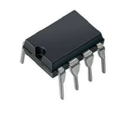
\includegraphics[width=0.2\textwidth]{Figures/Figure 3.10.png}
    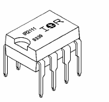
\includegraphics[width=0.17\textwidth]{Figures/Figure 3.11.png}
    \caption{High-Voltage Half-Bridge Gate Driver IC IR2111 Block Assignment.}
    \label{fig:gate_driver_ic}
\end{figure}

\renewcommand{\arraystretch}{1.4} % Provides clean vertical padding
\rowcolors{2}{white}{gray!8} % Alternating soft gray zebra stripes

\noindent % Prevents any accidental paragraph indentation shifts
\centerline{% Forces the entire text-width container into exact center alignment
\begin{tabularx}{\textwidth}{>{\bfseries}l X}
    \toprule
    Parameter & Specification \\
    \midrule
    Manufacturer & International Rectifier (now Infineon Technologies) \\
    Voltage Ratings & Operates up to $+600$ V with a high-side floating channel supply \\
    Output Current Capability & $0.5$ A sink and $0.25$ A source (typical values) \\
    Logic Compatibility & Logic input voltage is compatible with standard TTL/CMOS levels (0 V to $V_{CC}$), independent of the high-voltage supply rail channel \\
    Propagation Delay Parameters & Features a turn-on propagation delay of 750 ns and a turn-off propagation delay of 150 ns \\
    \bottomrule
\end{tabularx}%
}

\subsubsection{Application in the Project}
In this project, the IR2111 interfaces between the Arduino Uno's low-voltage PWM outputs and the IRFP260 MOSFETs used in the boost converter, buck converter, and two-quadrant chopper. Since the Arduino cannot supply enough current to switch the MOSFETs quickly, the IR2111 amplifies and level-shifts each PWM signal to drive the gates with fast, clean transitions and minimal switching loss. 

Its independent high-side and low-side channels, with built-in dead-time protection, make it especially suited to the two-quadrant chopper, where both switches must operate without overlap to avoid short-circuiting the DC bus. The floating high-side channel also allows proper switching even when the high-side MOSFET's source is not grounded.

% -------------------------------------------------------------------------
\subsection{Optocoupler – 6N139}

\subsubsection{Description and Key Specifications}
The 6N139 is a high-gain, split-Darlington output optocoupler designed to provide safe electrical isolation between low-voltage control circuits and high-voltage power electronic stages.

\begin{figure}[H]
    \centering
    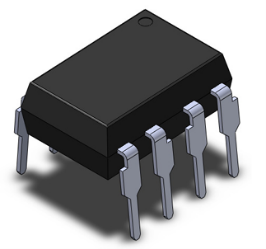
\includegraphics[width=0.2\textwidth]{Figures/Figure 3.12.png}
    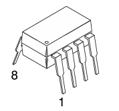
\includegraphics[width=0.2\textwidth]{Figures/Figure 3.13.png}
    \caption{6N139 High-Gain Darlington Optocoupler Package.}
    \label{fig:optocoupler}
\end{figure}

\begin{itemize}
    \item \textbf{Output Type:} Split-Darlington Transistor (provides an exceptionally high Current Transfer Ratio - CTR, typically exceeding 400\%).
    \item \textbf{Switching Capability:} Suitable for PWM frequencies in the low tens of kilohertz range (e.g., 10 kHz) when appropriately calibrated with a dynamic pull-down resistor.
    \item \textbf{Input Forward Voltage:} 1.4 V typical threshold.
    \item \textbf{Isolation Rating:} Up to $5000\text{ V}_{RMS}$ high galvanic isolation.
\end{itemize}

\subsubsection{Application in the Project}
In this project, the 6N139 optocoupler is placed between the Arduino Uno's PWM output and the input of the IR2111 gate driver IC, serving across various converter control channels (MPPT stage, boost converter, buck converter, and two-quadrant chopper). Its primary role is to \textit{electrically isolate the low-voltage microcontroller side from the high-voltage power electronics side}, since the gate driver and MOSFETs operate at higher voltage and current levels and are directly exposed to severe switching noise, ground bounce, and potential fault conditions.

The exceptionally high CTR of the 6N139's Darlington stage is critical for this application, as it allows the weak, milliampere-level 5V logic signal from the Arduino to deeply saturate the output transistor and robustly trigger the 12V gate drive stage. Furthermore, due to the specific pull-down wiring configuration utilized in the hardware, the 6N139 inherently acts as a logical inverter (a HIGH signal from the microcontroller pulls the isolated output LOW). This precise hardware behavior is actively compensated for within the embedded control firmware to maintain accurate duty-cycle regulation without introducing latency, preserving the responsiveness of the MPPT algorithm and the converter closed-loop control.
\newpage
% -------------------------------------------------------------------------
\subsection{MOSFET – IRFP260N}

\subsubsection{Description and Key Specifications}
The IRFP260N is an advanced N-channel power MOSFET utilizing HEXFET® technology, specifically optimized for high-speed, heavy-duty power switching applications requiring extremely low conduction losses.

\begin{figure}[H]
    \centering
    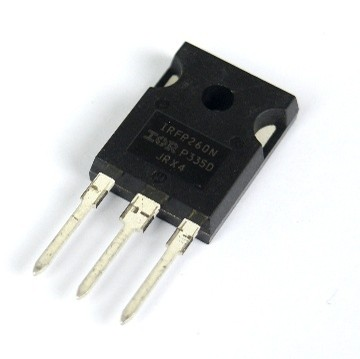
\includegraphics[width=0.2\textwidth]{Figures/3.14.jpg}
    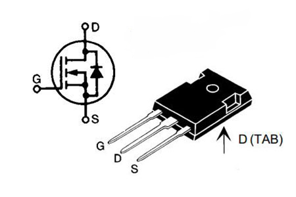
\includegraphics[width=0.35\textwidth]{Figures/3.144.png}
    \caption{IRFP260N Power MOSFET Schematic Symbol and TO-247AC Package Outline.}
    \label{fig:mosfet}
\end{figure}

\renewcommand{\arraystretch}{1.4} % Provides clean vertical padding
\rowcolors{2}{white}{gray!8} % Alternating soft gray zebra stripes

\noindent % Prevents any accidental paragraph indentation shifts
\centerline{% Forces the entire text-width container into exact center alignment
\begin{tabularx}{\textwidth}{>{\bfseries}l X}
    \toprule
    Parameter & Specification \\
    \midrule
    Manufacturer & Infineon Technologies / International Rectifier (IR) \\
    Drain-Source Breakdown Voltage ($V_{DS}$) & 200 V \\
    Continuous Drain Current ($I_D$) & 50 A (at $T_c = 25^\circ\text{C}$) \\
    On-State Channel Resistance ($R_{DS(on)}$) & $0.04\ \Omega$ at $V_{GS} = 10\text{ V}$ \\
    Gate Threshold Voltage Range & 2.0 V to 4.0 V \\
    \bottomrule
\end{tabularx}%
}

\subsubsection{Application in the Project}
The IRFP260N serves as the primary switching semiconductor in the bidirectional Two-Quadrant Chopper, as well as the independent boost and buck converter stages. Driven by the isolated IR2111 gate driver IC, it switches ON and OFF precisely at the 10 kHz duty cycle commanded by the microcontroller to regulate the microgrid's energy transfer. 

The selection of the "N" variant is critical to the system's thermodynamic stability. Its robust 200V/50A ratings provide an absolute safety margin against transient inductive spikes ($V = L \frac{di}{dt}$). More importantly, its ultra-low on-state resistance ($R_{DS(on)} = 0.04\ \Omega$) is the cornerstone of the Synchronous Rectification strategy utilized in the Two-Quadrant Chopper. By substituting standard freewheeling diodes with this actively driven MOSFET, conduction losses are drastically minimized, transitioning the thermal dissipation from a linear function to a quadratic resistive function. Coupled with the large TO-247AC package, this allows the power stages to operate efficiently under continuous 0.40A to high-current off-grid loads without necessitating complex forced-air cooling infrastructure.
\newpage
% -----------------------------------------
\subsection{Resistors}

\subsubsection{Description and Key Specifications}
Resistors are passive components used to limit current, divide voltage, and bias active components. In this project, resistors of different values and power ratings were used across the circuit—from low-power signal applications, like gate driver and optocoupler inputs, to higher-power applications, like voltage sensing and current limiting in the power stages.

\begin{figure}[H]
    \centering
    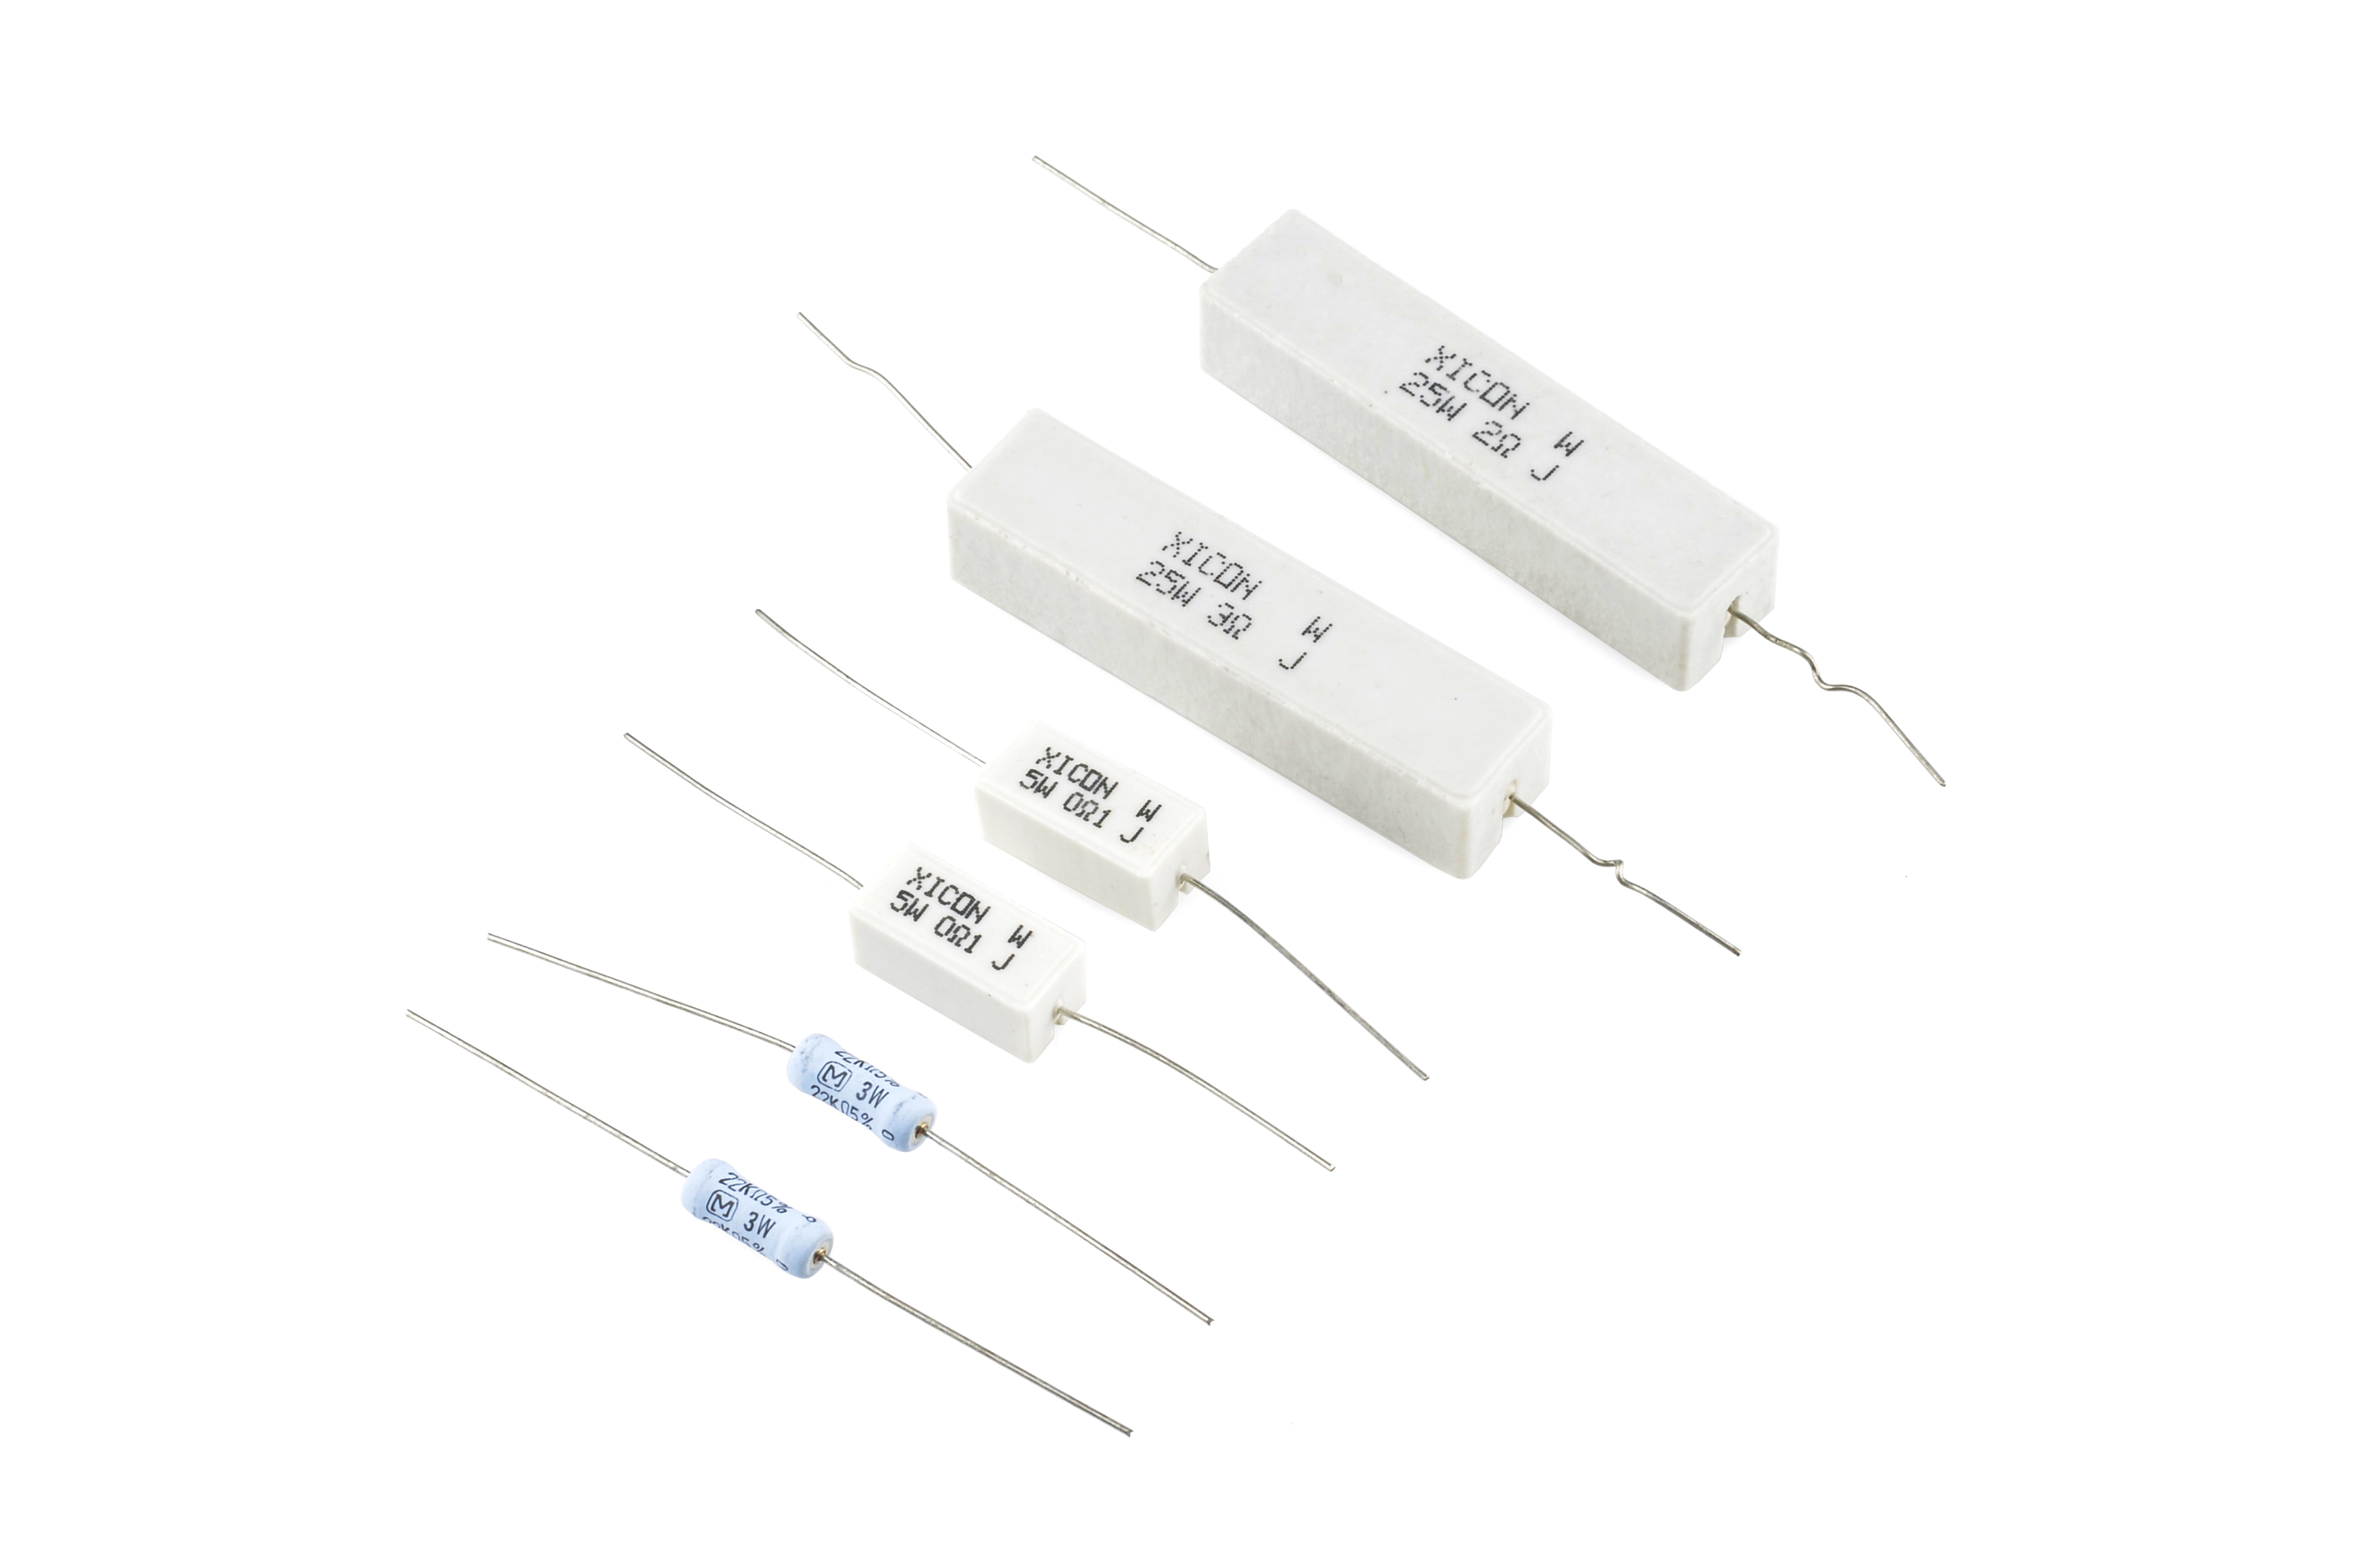
\includegraphics[width=0.4\textwidth]{Figures/res.jpg}
    \caption{Through-Hole Fixed Resistor Component Structure.}
    \label{fig:resistor}
\end{figure}

\renewcommand{\arraystretch}{1.4} % Provides clean vertical padding
\rowcolors{2}{white}{gray!8} % Alternating soft gray zebra stripes

\noindent % Prevents any accidental paragraph indentation shifts
\centerline{% Forces the entire text-width container into exact center alignment
\begin{tabularx}{\textwidth}{>{\bfseries}l X}
    \toprule
    Parameter & Specification \\
    \midrule
    Type & Fixed carbon-film / metal-film resistors (through-hole parameters) \\
    Resistance Values & Multiple values used (ranging from a few ohms up to several kilo-ohms), selected per circuit requirement \\
    Power Ratings & Multiple ratings used (1/4 W for signal-level circuits up to several watts for higher-current sections), selected based on expected power dissipation at each location \\
    Tolerance Value & $\pm5\%$ standard margin for general-purpose applications \\
    \bottomrule
\end{tabularx}%
}

\subsubsection{Application in the Project}
In this project, resistors were used in several roles depending on the circuit stage:
\begin{itemize}
    \item \textbf{Pull-up/Pull-down and Biasing:} Used at the inputs/outputs of the optocoupler (6N137M) and gate driver IC (IR2111) to ensure proper logic-level operation and prevent floating signals.
    \item \textbf{Voltage Division:} Used in sensing circuits to scale down higher voltages (e.g., PV array or battery voltage) to levels safely readable by the Arduino's analog input pins.
    \item \textbf{Current Limiting:} Used to protect LEDs, optocoupler input diodes, and other low-power components from excessive current.
    \item \textbf{Current Sensing:} Higher-power resistors (shunt-type) were used where applicable to sense current flow in the power stages, generating a small voltage drop proportional to current for feedback purposes.
\end{itemize}

% -------------------------------------------------------------------------
\subsection{Inductors}

\subsubsection{Description and Key Specifications}
Power inductors are passive components used to store energy in a magnetic field and smooth current flow. In this project, power inductors of different inductance values and current ratings were used as the main energy-storage elements in the boost converter, buck converter, and two-quadrant chopper.

\begin{figure}[H]
    \centering
    \begin{minipage}{0.48\textwidth}
        \centering
        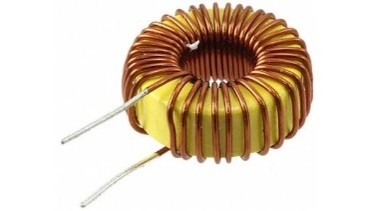
\includegraphics[width=0.8\textwidth]{Figures/Picture16.jpg}
        \caption{Toroidal Inductor Core}
    \end{minipage}\hfill
    \begin{minipage}{0.48\textwidth}
        \centering
        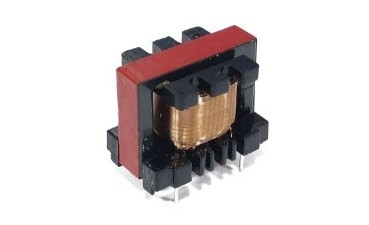
\includegraphics[width=0.7\textwidth]{Figures/Picture15.jpg}
        \caption{Wound Ferrite Inductor}
    \end{minipage}
\end{figure}

\begin{itemize}
    \item \textbf{Type:} Wound power inductors (core type selected according to current and switching frequency requirements).
    \item \textbf{Inductance Parameters:} Multiple values used, depending on the specific converter stage and its switching frequency.
    \item \textbf{Current Ratings:} Selected based on the maximum current expected to flow through each inductor without saturating the magnetic core boundaries.
\end{itemize}

\subsubsection{Application in the Project}
The power inductors form the main energy-storage element in the boost converter, buck converter, and two-quadrant chopper, storing energy from the source during the switch's ON state and releasing it to the load during the OFF state—this charge/discharge cycle is what enables the voltage step-up/step-down action of each converter. Selecting the appropriate inductance and current rating at each stage was necessary to ensure efficient energy transfer while keeping current ripple within acceptable limits.
\newpage
% -------------------------------------------------------------------------
\subsection{Capacitors}

\subsubsection{Description and Key Specifications}
Capacitors are passive components used to store electrical energy and smooth voltage variations. In this project, capacitors of different capacitance values and voltage ratings were used across the circuit—from small-value capacitors for decoupling and filtering at IC supply pins, to higher-value capacitors used for input/output filtering in the boost converter, buck converter, and two-quadrant chopper.

\begin{figure}[H]
    \centering
    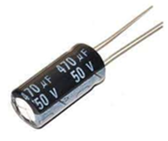
\includegraphics[width=0.4\textwidth]{Figures/Picture17.png}
    \caption{Through-Hole Radial Electrolytic Filter Capacitor Board Component.}
    \label{fig:capacitor}
\end{figure}

\begin{itemize}
    \item \textbf{Type:} Electrolytic and ceramic capacitors (through-hole style configurations).
    \item \textbf{Capacitance Range:} Multiple values used, ranging from sub-microfarad ceramic capacitors for noise decoupling up to higher-value electrolytic capacitors for converter filtering.
    \item \textbf{Voltage Safe Limits:} Selected according to the maximum voltage present at each point in the circuit, with an appropriate safety margin index.
\end{itemize}

\subsubsection{Application in the Project}
\begin{itemize}
    \item \textbf{Output Filtering:} Capacitors are placed at the output of each converter stage to smooth the switched voltage waveform, reducing ripple and providing a stable DC output to the next stage (battery, EV charging output, etc.).
    \item \textbf{Input Filtering:} Capacitors are also used at the input of converter stages to filter switching noise from feeding back into the PV array or battery source.
    \item \textbf{Decoupling:} Small-value capacitors are placed close to the supply pins of ICs, such as the IR2111 gate driver and the LM7812 regulator, to filter high-frequency noise and stabilize the supply voltage during fast switching transients.
\end{itemize}